% =====================================================================
% Herança Ativa para Geração Sintética de Desinformação:
% um Estudo Controlado Multi-domínio
% Artigo IEEEtran (conference). Cobre: RQs, 4 domínios, baselines
% Real/Static, estudo controlado de 4 regras de herança, custo,
% figuras Pareto, diagnóstico real-vs-sintético e limitações.
% =====================================================================
\documentclass[conference]{IEEEtran}
\usepackage[utf8]{inputenc}
\usepackage[T1]{fontenc}
\usepackage{cite}
\usepackage{amsmath,amssymb,amsfonts}
\usepackage{graphicx}
\usepackage{textcomp}
\usepackage{xcolor}
\usepackage{booktabs}
\usepackage[hidelinks]{hyperref}
\usepackage{url}
\usepackage{balance}
\graphicspath{{./images/}{../figures/revision/}{./}}
\setlength{\textfloatsep}{8pt plus 1pt minus 1pt}
\setlength{\intextsep}{6pt plus 1pt minus 1pt}
\setlength{\floatsep}{6pt plus 1pt minus 1pt}
\widowpenalty=10000
\clubpenalty=10000

\begin{document}

\title{Heran\c{c}a Ativa para Gera\c{c}\~ao Sint\'etica de Desinforma\c{c}\~ao:\\um Estudo Controlado Multi-dom\'inio}

\author{\IEEEauthorblockN{Eduardo Alexandre de Amorim\textsuperscript{1} e Cleber Zanchettin\textsuperscript{1}}
\IEEEauthorblockA{\textsuperscript{1}Centro de Inform\'atica, Universidade Federal de Pernambuco (CIn/UFPE), Recife, PE, Brasil\\
eaa5@cin.ufpe.br, cz@cin.ufpe.br}}

\maketitle

\begin{abstract}
A escassez de exemplos rotulados de desinforma\c{c}\~ao limita classificadores robustos, enquanto a gera\c{c}\~ao sint\'etica indiscriminada pode introduzir redund\^ancia, artefatos e ru\'ido. Este trabalho prop\~oe a \emph{Heran\c{c}a Ativa} (ActiveInheritance): um processo c\'iclico em que um modelo de linguagem gera candidatos falsos e um avaliador adversarial, que combina o erro, a incerteza e a diversidade do classificador downstream, seleciona apenas o top-$k$ para ser herdado no ciclo seguinte de treino. Para isolar o efeito da regra de sele\c{c}\~ao do volume gerado e da pol\'itica de treino, conduzimos um estudo controlado em quatro dom\'inios do portugu\^es (Fake.br, FakeWhatsApp.Br, COVID19.BR e FACTCK.BR). Nos quatro dom\'inios, uma \'unica gera\c{c}\~ao zero-shot por cen\'ario e semente \'e re-executada offline com quatro regras de heran\c{c}a: herdar tudo (\emph{All}), uma amostra aleat\'oria (\emph{Random-}k), o score top-$k$ (\emph{Score-}k) e o gate invertido (\emph{Easy-}k), em tr\^es n\'iveis de escassez e dez sementes (440 runs). Os resultados mostram que o score n\~ao domina a sele\c{c}\~ao aleat\'oria, que o efeito observado \'e sobretudo curadoria de volume, e que a sele\c{c}\~ao guiada s\'o agrega em regimes de dificuldade intermedi\'aria; a pondera\c{c}\~ao de classes e o limiar ajustado respondem pela maior parte do ganho. Al\'em disso, um classificador linear distingue o texto sint\'etico do real com AUC $=$ 1{,}000, indicando um atalho estil\'istico que a sele\c{c}\~ao n\~ao elimina.
\end{abstract}

\begin{IEEEkeywords}
data-centric AI, synthetic data, misinformation, active inheritance, controlled study, Portuguese NLP
\end{IEEEkeywords}

\section{Introdu\c{c}\~ao}

Detectar desinforma\c{c}\~ao em texto \'e uma classifica\c{c}\~ao bin\'aria (verdadeiro \emph{vs.} falso) que sofre de escassez e desbalanceamento da classe de interesse: os exemplos falsos s\~ao poucos, mudam de dom\'inio rapidamente e custam caro para rotular. Modelos de linguagem permitem produzir dados sint\'eticos, mas volume n\~ao garante utilidade: gera\c{c}\~oes podem repetir templates, afastar-se da distribui\c{c}\~ao real e receber r\'otulos presumidos incorretos \cite{shumailov2024collapse}. O ponto fr\'agil \'e, portanto, a sele\c{c}\~ao do que gerar e do que usar.

Este trabalho prop\~oe a \emph{Heran\c{c}a Ativa} (ActiveInheritance), inspirada na perspectiva \emph{data-centric} do Profile2Gen \cite{souza2025profile2gen}. Em ciclos, um gerador produz um lote de textos falsos; um avaliador pontua cada candidato pelo erro do classificador downstream, pela incerteza da predi\c{c}\~ao e pela diversidade em rela\c{c}\~ao ao pool herdado; apenas o top-$k$ \'e herdado e o classificador \'e retreinado sobre os dados reais somados ao pool herdado. A hip\'otese \'e a de treino deliberado: gastar o or\c{c}amento com exemplos que o modelo ainda acha dif\'iceis, n\~ao com exemplos f\'aceis ou repetitivos.

As perguntas de pesquisa (RQs) s\~ao:

\begin{itemize}
\item \textbf{RQ1 (qualidade).} Dados os mesmos candidatos, a sele\c{c}\~ao pelo score de erro/incerteza/diversidade produz um conjunto herdado mais \'util que uma amostra aleat\'oria?
\item \textbf{RQ2 (efici\^encia).} A sele\c{c}\~ao reduz o custo de gera\c{c}\~ao por unidade de desempenho?
\item \textbf{RQ3 (robustez).} O m\'etodo se mant\'em sob escassez extrema da classe falsa (5\%)?
\end{itemize}

As contribui\c{c}\~oes s\~ao: (i) um pipeline completo de heran\c{c}a ativa para o portugu\^es; (ii) um estudo controlado multi-dom\'inio que fixa os candidatos e varia apenas a regra de heran\c{c}a; (iii) baselines Real e Static com pondera\c{c}\~ao de classes e limiar ajustado; (iv) an\'alise de custo, diversidade, fidelidade e artefatos; e (v) resultados negativos que delimitam \emph{quando} o m\'etodo funciona.

\section{Trabalhos Relacionados}

\emph{Gera\c{c}\~ao de dados sint\'eticos.} ZeroGen \cite{ye2022zerogen} e ProGen \cite{meng2022progen} mostram que corpora gerados por LLMs podem substituir dados de treino em tarefas de NLP; SunGen \cite{gao2023sungen} refina a gera\c{c}\~ao com auto-orienta\c{c}\~ao para reduzir ru\'ido. Esses trabalhos, por\'em, n\~ao comparam regras de sele\c{c}\~ao sobre um mesmo lote de candidatos.

\emph{Sele\c{c}\~ao ativa e cartografia.} O \emph{active learning} \cite{settles2009active} seleciona inst\^ancias reais para anota\c{c}\~ao; aqui selecionamos inst\^ancias \emph{sint\'eticas} para heran\c{c}a. A cartografia de datasets \cite{swayamdipta2020cartography} usa din\^amicas de treino (erro e confian\c{c}a) para diagnosticar regi\^oes f\'aceis, amb\'iguas e dif\'iceis; nosso score \'e uma vers\~ao online dessa ideia, acrescida de diversidade.

\emph{Profile2Gen.} O trabalho de refer\^encia \cite{souza2025profile2gen} formaliza uma abordagem \emph{data-centric} para dados tabulares, removendo \emph{hard samples} no p\'os-processamento. Invertemos o desenho: herdamos os candidatos que o classificador acha dif\'iceis e incertos, em texto/classifica\c{c}\~ao.

\section{M\'etodo}

\subsection{Loop de Heran\c{c}a Ativa}

Seja $D_0 = \{(\mathbf{x}_i, y_i)\}$ o treino real escasso, com $y_i \in \{0,1\}$ ($1$ = falso). A cada ciclo $t=0,\dots,T-1$: (1) um gerador $G$ produz um lote de candidatos falsos $\hat{X}_t$ de tamanho $b$; (2) o avaliador pontua cada candidato por
\begin{equation}
s(\hat{\mathbf{x}}) = w_e\,e(\hat{\mathbf{x}}) + w_u\,u(\hat{\mathbf{x}}) + w_d\,d(\hat{\mathbf{x}}; H),
\label{eq:score}
\end{equation}
em que $e$ \'e o erro do classificador (log-loss da classe falsa, normalizado por min-max no lote), $u$ a incerteza (entropia bin\'aria normalizada), $d$ a diversidade ($1 - \max$ similaridade de cosseno contra o pool herdado $H$, com $d{=}1$ no primeiro ciclo), e $(w_e, w_u, w_d) = (0{,}4, 0{,}4, 0{,}2)$; (3) apenas o top-$k$ \'e herdado; (4) o classificador \'e retreinado em $D_0 \cup H$.

\subsection{Baselines e regras de heran\c{c}a}

\begin{itemize}
\item \textbf{Real}: BERTimbau treinado apenas nos dados reais (zero sint\'eticos);
\item \textbf{Static}: o gerador produz $N$ textos e todos entram no treino, sem sele\c{c}\~ao;
\item \textbf{ActiveInheritance (AI)}: somente o top-$k$ pela Equa\c{c}\~ao~\ref{eq:score} \'e herdado.
\end{itemize}

Para isolar a regra de sele\c{c}\~ao, fixamos os candidatos e comparamos quatro regras sobre os \emph{mesmos} lotes:

\begin{itemize}
\item \textbf{All}: herda todos os candidatos (sem sele\c{c}\~ao);
\item \textbf{Random-}k: herda $k$ candidatos sorteados uniformemente;
\item \textbf{Score-}k: herda os $k$ de maior $s(\cdot)$;
\item \textbf{Easy-}k: herda os $k$ de menor $s(\cdot)$ (gate invertido, como controle negativo).
\end{itemize}

\subsection{Pol\'itica de treino}

Para separar qualidade sint\'etica de pol\'itica de treino, todos os bra\c{c}os usam a mesma pol\'itica: pondera\c{c}\~ao de classes por ajuste, limiar de decis\~ao ajustado na valida\c{c}\~ao e, no fim, um BERTimbau novo treinado do zero em $D_0 \cup H$ (o retreino por ciclo usa \emph{warm-start}; o treino final \'e do zero). O limiar \'e escolhido maximizando F1 na valida\c{c}\~ao; o teste \'e usado uma \'unica vez.

\section{Configura\c{c}\~ao Experimental}

\subsection{Datasets}

A Tabela~\ref{tab:datasets} resume os quatro dom\'inios. O Fake.br \cite{monteiro2018fakebr} cont\'em not\'icias em portugu\^es pr\'e-processadas; criamos escassez somente no treino (10\% e 5\% de exemplos falsos), com valida\c{c}\~ao fixa e holdout balanceado. FakeWhatsApp.Br \cite{cabral2021fakewhatsapp} e COVID19.BR \cite{cabral2020covid19br} s\~ao mensagens reais de WhatsApp rotuladas manualmente, com split temporal (FakeWhatsApp.Br: treino julho a agosto de 2018, valida\c{c}\~ao setembro, teste outubro; COVID19.BR: treino mar\c{c}o a abril de 2020, valida\c{c}\~ao 08 a 09 de junho, teste 10 a 12 de junho). FACTCK.BR \cite{moreno2019factckbr} cont\'em claims verificados por ag\^encias de checagem, com texto = \texttt{claimReviewed} (o \texttt{reviewBody} foi descartado por declarar o veredito), binariza\c{c}\~ao estrita e split aleat\'orio estratificado 70/15/15. Em cada dom\'inio, variamos a escassez da classe falsa no treino: full, 10\% e 5\% (mantendo todos os exemplos verdadeiros).

\begin{table}[t]
\caption{Caracter\'isticas dos quatro dom\'inios.}\label{tab:datasets}
\centering
\footnotesize
\setlength{\tabcolsep}{4pt}
\begin{tabular}{@{}lllll@{}}
\toprule
Dom\'inio & G\^enero & Texto & Prior fake & Split \\
\midrule
Fake.br & not\'icia & pr\'e-proc. & balanceado & aleat. fixa \\
FakeWhatsApp.Br & WhatsApp & raw & minorit\'ario & temporal \\
COVID19.BR & WhatsApp & raw & minorit\'ario ($\approx$1:2{,}5) & temporal \\
FACTCK.BR & claims & raw & majorit\'ario & aleat. estrat. \\
\bottomrule
\end{tabular}
\end{table}

\subsection{Protocolo}

\emph{Fake.br.} Al\'em dos bra\c{c}os Real, Static ($N{=}158$) e AI (replay com pondera\c{c}\~ao de classes e limiar ajustado sobre os pools hist\'oricos), o Fake.br tamb\'em entrou no estudo controlado abaixo, com candidates zero-shot gerados no prompt v2 e normaliza\c{c}\~ao aproximada do sint\'etico (\texttt{normalize\_fakebr}).

\emph{Estudo controlado (quatro dom\'inios).} Para cada cen\'ario (dom\'inio $\times$ escassez) e semente, realizamos uma \'unica gera\c{c}\~ao zero-shot com \texttt{deepseek-chat} ($T{=}5$ ciclos, lote de 64, teto de 100 mil tokens, top-$k{=}16$), prompt v4 (mensagem de WhatsApp anti-template) nos dom\'inios WhatsApp e v2 (not\'icia/claim) no FACTCK.BR e no Fake.br. Os lotes s\~ao congelados em \texttt{candidates.json} e, offline, as quatro regras s\~ao re-executadas sobre os \emph{mesmos} candidatos, sem nova chamada \`a API. O classificador downstream \'e o BERTimbau \cite{souza2020bertimbau} (\texttt{neuralmind/bert-base-portuguese-cased}), 3 \'epocas por ajuste, batch 16, comprimento m\'aximo 256. As sementes s\~ao 42 a 51 ($n{=}10$): a semente muda a inicializa\c{c}\~ao, a ordem de treino e a amostragem estoc\'astica do servidor LLM, n\~ao os splits (fixos) nem a valida\c{c}\~ao.

\subsection{M\'etricas}

Reportamos F1, precis\~ao e recall da classe falsa, PR-AUC e ROC-AUC, m\'edia e desvio populacional entre sementes, tokens de entrada/sa\'ida e custo estimado, similaridade m\'edia do pool, TTR de trigramas e dist\^ancia de Wasserstein como proxy de fidelidade (n\~ao de veracidade). Com $n{=}10$, o menor $p$ poss\'ivel do Wilcoxon bilateral pareado \'e $\approx$0{,}002.

\section{Resultados}

\subsection{Fake.br}

A Tabela~\ref{tab:fakebr} reporta os bra\c{c}os Real, Static e AI com pondera\c{c}\~ao e limiar ajustado. No cen\'ario 10\%, o AI alcan\c{c}a o maior F1 (0{,}934 $\pm$ 0{,}002); no 5\%, os tr\^es bra\c{c}os empatam e o sint\'etico deixa de ajudar, ecoando a depend\^encia de um learner inicial competente. Historicamente, a compara\c{c}\~ao descritiva Static-79 (0{,}852 $\pm$ 0{,}034) \emph{vs.} AI com 80 herdados (0{,}924 $\pm$ 0{,}007) sugere um ganho de $\approx$0{,}072, mas n\~ao atribu\'imos causalidade ao score: gera\c{c}\~ao, prompt e ciclos diferem entre as condi\c{c}\~oes.

\begin{table}[t]
\caption{F1 e recall (m\'edia $\pm$ desvio, $n{=}3$) no Fake.br, com pondera\c{c}\~ao de classes e limiar ajustado.}\label{tab:fakebr}
\centering
\footnotesize
\setlength{\tabcolsep}{4pt}
\begin{tabular}{@{}llcc@{}}
\toprule
Cen\'ario & Bra\c{c}o & F1 & Recall \\
\midrule
10\% & Real & 0.920 $\pm$ 0.010 & 0.861 $\pm$ 0.019 \\
10\% & Static (158) & 0.911 $\pm$ 0.018 & 0.841 $\pm$ 0.031 \\
10\% & AI & 0.934 $\pm$ 0.002 & 0.891 $\pm$ 0.003 \\
5\% & Real & 0.897 $\pm$ 0.012 & 0.819 $\pm$ 0.018 \\
5\% & Static (158) & 0.899 $\pm$ 0.011 & 0.822 $\pm$ 0.018 \\
5\% & AI & 0.884 $\pm$ 0.016 & 0.797 $\pm$ 0.027 \\
\bottomrule
\end{tabular}
\end{table}

\subsection{Estudo controlado}

A Tabela~\ref{tab:f1} reporta F1 por dom\'inio, cen\'ario e regra; a Tabela~\ref{tab:aux} traz recall, PR-AUC e o n\'umero de sint\'eticos herdados. O bra\c{c}o \emph{All} herda $\approx$302 a 313 sint\'eticos; os demais herdam 80.

\begin{table*}[t]
\caption{F1 (teste) por dom\'inio, cen\'ario e regra de heran\c{c}a. $n{=}10$ sementes.}\label{tab:f1}
\centering
\footnotesize
\setlength{\tabcolsep}{6pt}
\begin{tabular}{@{}llcccc@{}}
\toprule
Dom\'inio & Cen. & All & Random-k & Score-k & Easy-k \\
\midrule
FakeWhatsApp.Br & full & 0.707 $\pm$ 0.029 & 0.721 $\pm$ 0.010 & 0.721 $\pm$ 0.017 & 0.722 $\pm$ 0.012 \\
FakeWhatsApp.Br & 10\% & 0.440 $\pm$ 0.161 & 0.587 $\pm$ 0.125 & 0.579 $\pm$ 0.137 & 0.582 $\pm$ 0.103 \\
FakeWhatsApp.Br & 5\% & 0.405 $\pm$ 0.130 & 0.463 $\pm$ 0.175 & 0.411 $\pm$ 0.188 & 0.419 $\pm$ 0.161 \\
COVID19.BR & full & 0.849 $\pm$ 0.023 & 0.847 $\pm$ 0.025 & 0.858 $\pm$ 0.022 & 0.855 $\pm$ 0.012 \\
COVID19.BR & 10\% & 0.666 $\pm$ 0.120 & 0.655 $\pm$ 0.125 & 0.728 $\pm$ 0.072 & 0.708 $\pm$ 0.068 \\
COVID19.BR & 5\% & 0.567 $\pm$ 0.122 & 0.691 $\pm$ 0.056 & 0.692 $\pm$ 0.070 & 0.639 $\pm$ 0.125 \\
FACTCK.BR & full & 0.926 $\pm$ 0.012 & 0.925 $\pm$ 0.009 & 0.930 $\pm$ 0.011 & 0.922 $\pm$ 0.012 \\
FACTCK.BR & 10\% & 0.840 $\pm$ 0.056 & 0.936 $\pm$ 0.007 & 0.934 $\pm$ 0.008 & 0.937 $\pm$ 0.006 \\
FACTCK.BR & 5\% & 0.785 $\pm$ 0.062 & 0.935 $\pm$ 0.008 & 0.936 $\pm$ 0.008 & 0.934 $\pm$ 0.006 \\
Fake.br & 10\% & 0.917 $\pm$ 0.014 & 0.922 $\pm$ 0.012 & 0.923 $\pm$ 0.014 & 0.920 $\pm$ 0.010 \\
Fake.br & 5\% & 0.872 $\pm$ 0.025 & 0.874 $\pm$ 0.016 & 0.880 $\pm$ 0.020 & 0.871 $\pm$ 0.015 \\
\bottomrule
\end{tabular}
\end{table*}

\begin{table*}[t]
\caption{Recall e PR-AUC (m\'edia) da classe falsa e n\'umero de sint\'eticos herdados ($n{=}10$).}\label{tab:aux}
\centering
\footnotesize
\setlength{\tabcolsep}{6pt}
\begin{tabular}{@{}lllccc@{}}
\toprule
Dom\'inio & Cen. & Bra\c{c}o & Recall & PR-AUC & n\_synth \\
\midrule
FakeWhatsApp.Br & full & all & 0.758 & 0.751 & 302 \\
FakeWhatsApp.Br & full & random-k & 0.804 & 0.762 & 80 \\
FakeWhatsApp.Br & full & score-k & 0.811 & 0.758 & 80 \\
FakeWhatsApp.Br & full & easy-k & 0.797 & 0.761 & 80 \\
FakeWhatsApp.Br & 10\% & all & 0.358 & 0.665 & 302 \\
FakeWhatsApp.Br & 10\% & random-k & 0.571 & 0.679 & 80 \\
FakeWhatsApp.Br & 10\% & score-k & 0.559 & 0.675 & 80 \\
FakeWhatsApp.Br & 10\% & easy-k & 0.548 & 0.690 & 80 \\
FakeWhatsApp.Br & 5\% & all & 0.315 & 0.634 & 302 \\
FakeWhatsApp.Br & 5\% & random-k & 0.437 & 0.631 & 80 \\
FakeWhatsApp.Br & 5\% & score-k & 0.369 & 0.626 & 80 \\
FakeWhatsApp.Br & 5\% & easy-k & 0.350 & 0.625 & 80 \\
COVID19.BR & full & all & 0.852 & 0.893 & 302 \\
COVID19.BR & full & random-k & 0.860 & 0.894 & 80 \\
COVID19.BR & full & score-k & 0.863 & 0.895 & 80 \\
COVID19.BR & full & easy-k & 0.869 & 0.894 & 80 \\
COVID19.BR & 10\% & all & 0.592 & 0.815 & 302 \\
COVID19.BR & 10\% & random-k & 0.561 & 0.825 & 80 \\
COVID19.BR & 10\% & score-k & 0.666 & 0.823 & 80 \\
COVID19.BR & 10\% & easy-k & 0.631 & 0.832 & 80 \\
COVID19.BR & 5\% & all & 0.447 & 0.798 & 302 \\
COVID19.BR & 5\% & random-k & 0.620 & 0.803 & 80 \\
COVID19.BR & 5\% & score-k & 0.621 & 0.800 & 80 \\
COVID19.BR & 5\% & easy-k & 0.547 & 0.800 & 80 \\
FACTCK.BR & full & all & 0.955 & 0.970 & 313 \\
FACTCK.BR & full & random-k & 0.957 & 0.968 & 80 \\
FACTCK.BR & full & score-k & 0.962 & 0.966 & 80 \\
FACTCK.BR & full & easy-k & 0.944 & 0.967 & 80 \\
FACTCK.BR & 10\% & all & 0.776 & 0.963 & 312 \\
FACTCK.BR & 10\% & random-k & 0.989 & 0.963 & 80 \\
FACTCK.BR & 10\% & score-k & 0.979 & 0.960 & 80 \\
FACTCK.BR & 10\% & easy-k & 0.985 & 0.963 & 80 \\
FACTCK.BR & 5\% & all & 0.686 & 0.951 & 312 \\
FACTCK.BR & 5\% & random-k & 0.986 & 0.955 & 80 \\
FACTCK.BR & 5\% & score-k & 0.988 & 0.957 & 80 \\
FACTCK.BR & 5\% & easy-k & 0.981 & 0.956 & 80 \\
Fake.br & 10\% & all & 0.859 & 0.983 & 312 \\
Fake.br & 10\% & random-k & 0.873 & 0.983 & 80 \\
Fake.br & 10\% & score-k & 0.873 & 0.987 & 80 \\
Fake.br & 10\% & easy-k & 0.882 & 0.987 & 80 \\
Fake.br & 5\% & all & 0.781 & 0.973 & 311 \\
Fake.br & 5\% & random-k & 0.784 & 0.975 & 80 \\
Fake.br & 5\% & score-k & 0.792 & 0.979 & 80 \\
Fake.br & 5\% & easy-k & 0.777 & 0.978 & 80 \\
\bottomrule
\end{tabular}
\end{table*}

\subsection{Custo e figuras}

Cada gera\c{c}\~ao zero-shot consome $\approx$99{,}5 mil tokens ($\approx$36 mil de entrada e $\approx$63 mil de sa\'ida), custando $\approx$\$0{,}08 por cen\'ario/semente. Com $\approx$320 candidatos, isso d\'a $\approx$311 tokens por candidato (gera\c{c}\~ao compartilhada pelos quatro bra\c{c}os; o custo de gera\c{c}\~ao \'e pago uma vez e reutilizado offline). A Figura~\ref{fig:nsynth} mostra o Pareto F1 $\times$ n\'umero de sint\'eticos no cen\'ario full: \emph{All} usa $\approx$302 a 313 textos, enquanto os bra\c{c}os curados usam 80 com F1 semelhante ou superior.

\begin{figure*}[t]
\centering
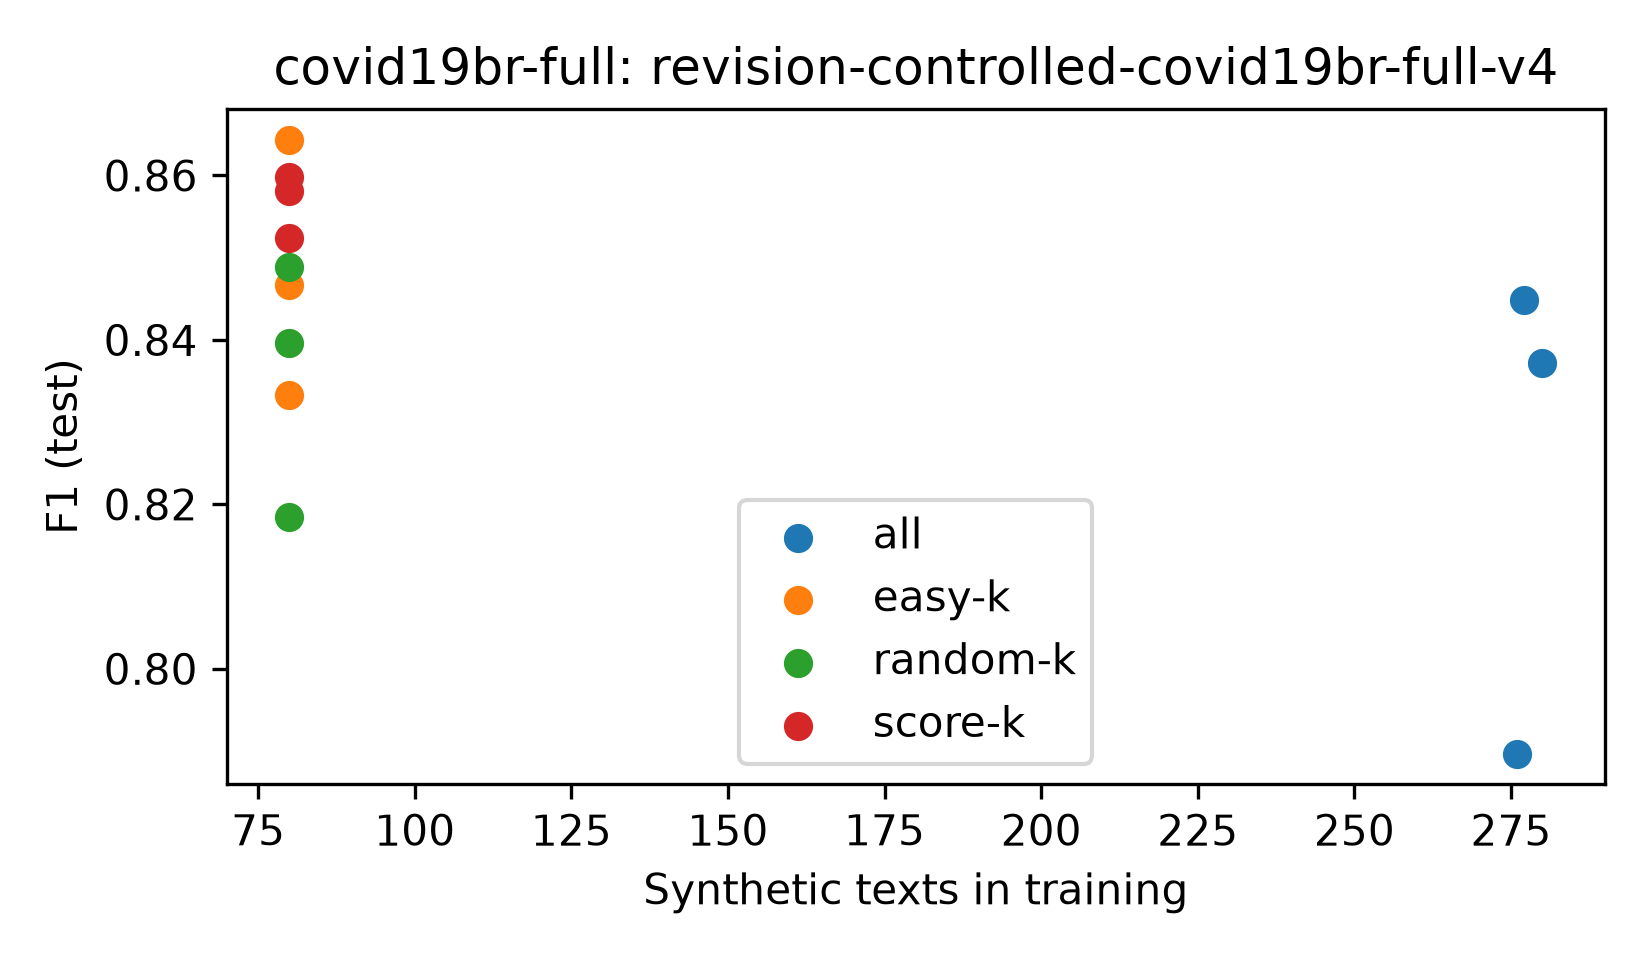
\includegraphics[width=0.32\textwidth]{revision-controlled-covid19br-full-v4-covid19br-full-f1-vs-n_synthetic-20261026T120542Z.png}\hfill
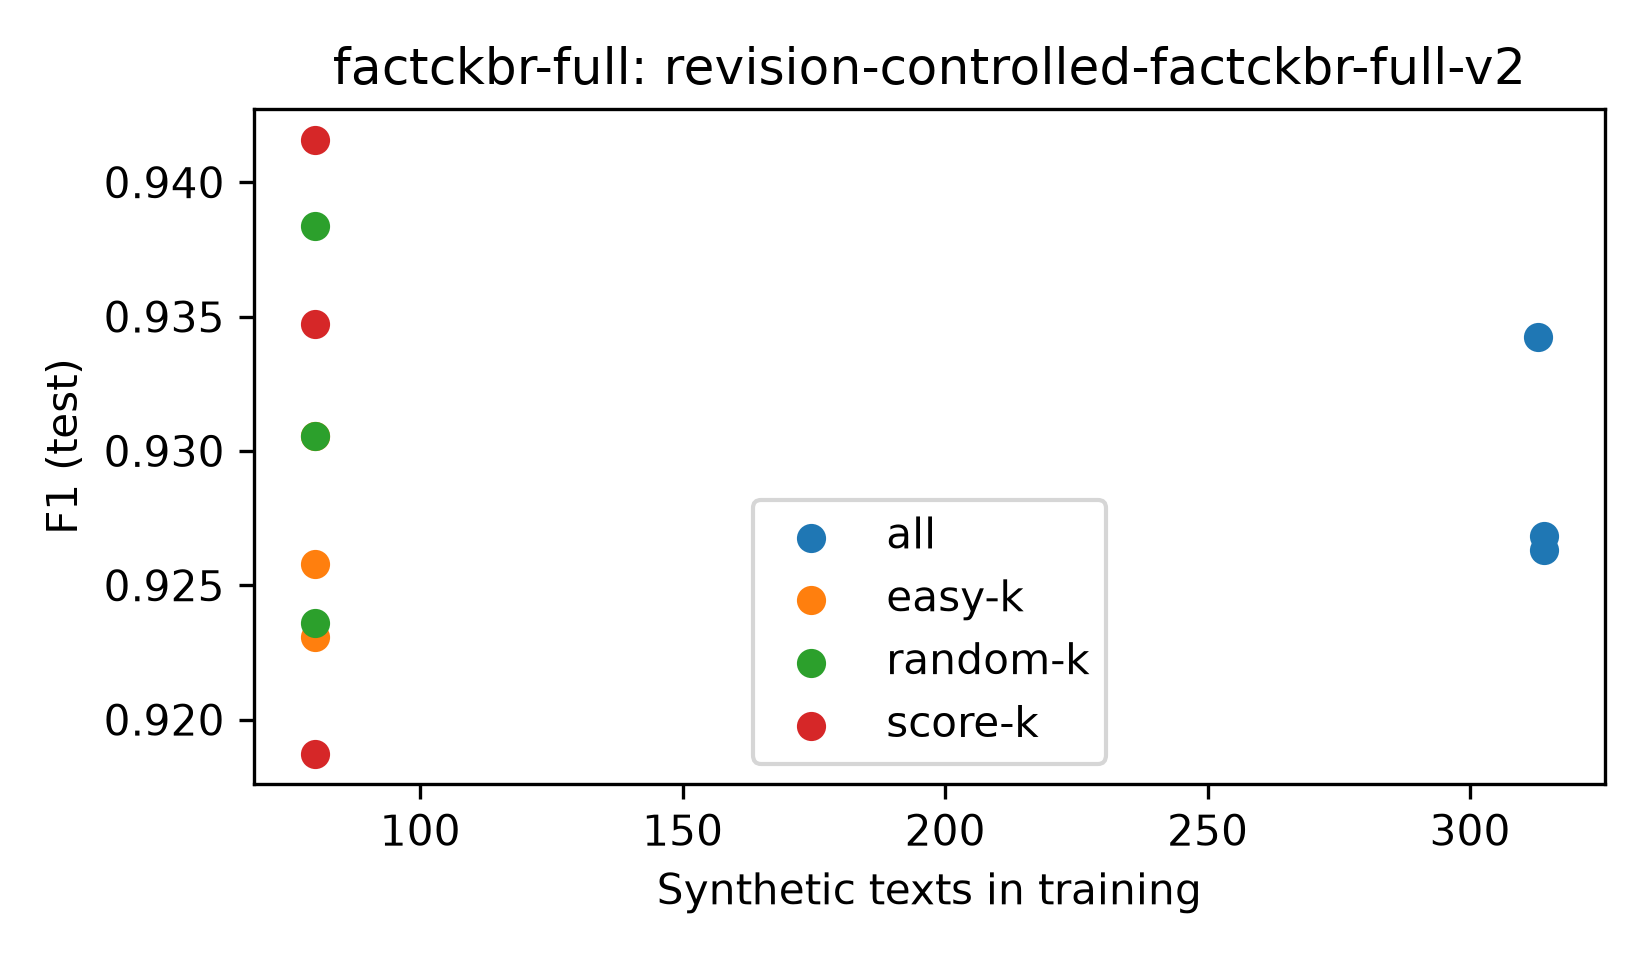
\includegraphics[width=0.32\textwidth]{revision-controlled-factckbr-full-v2-factckbr-full-f1-vs-n_synthetic-20261026T120546Z.png}\hfill
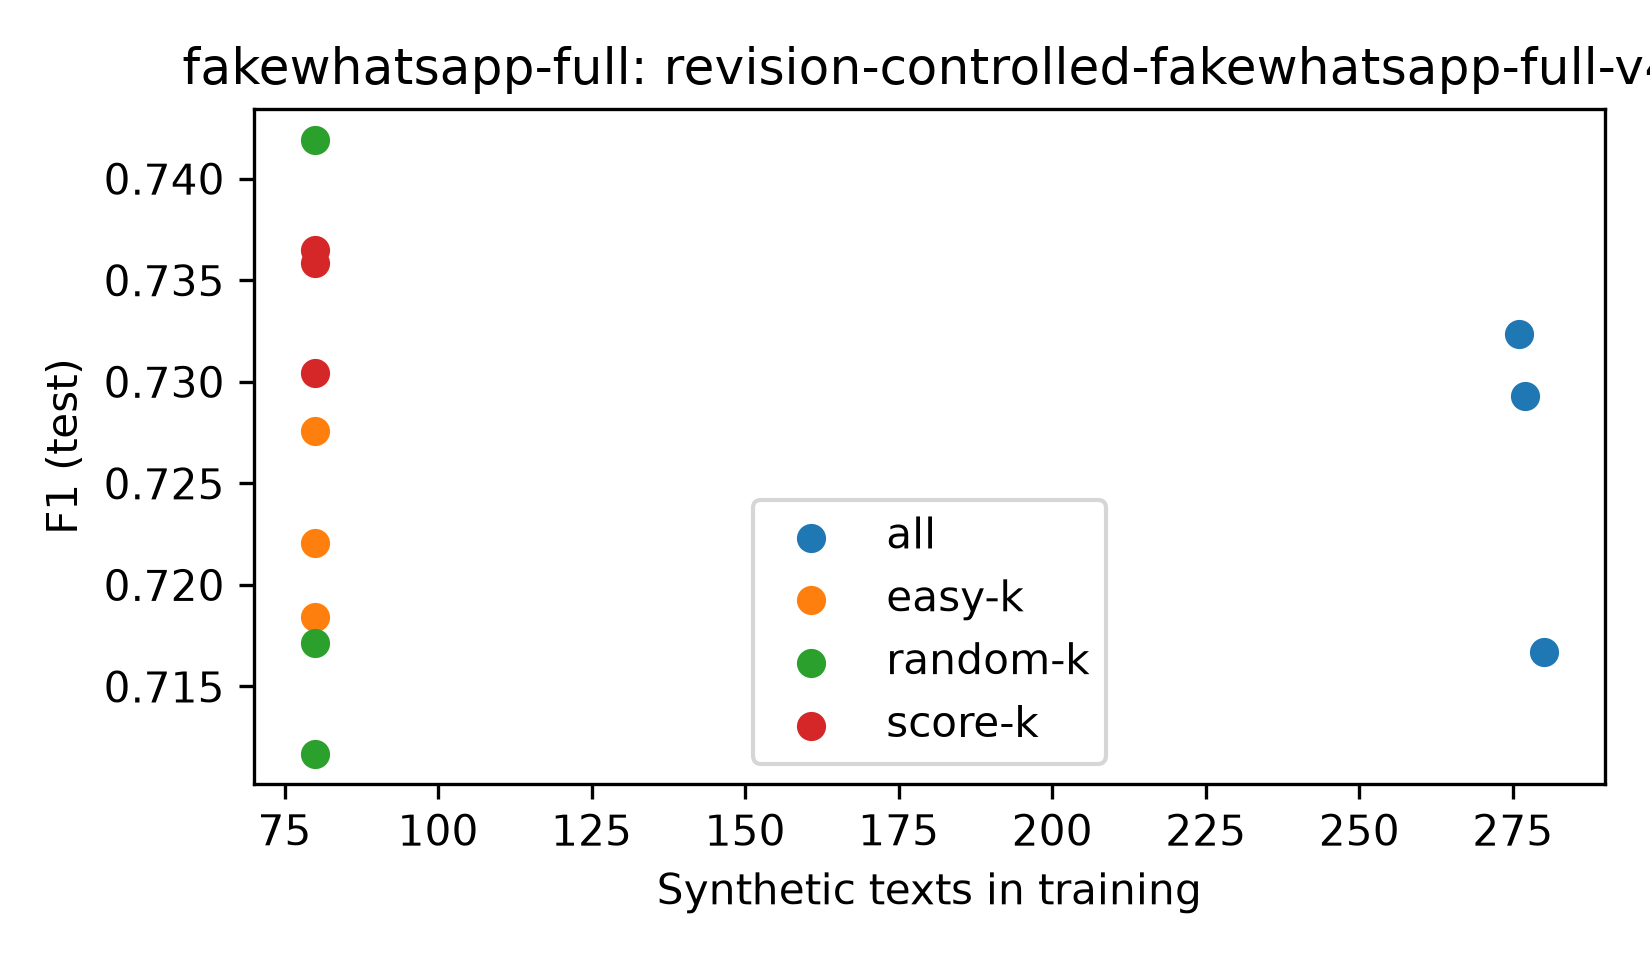
\includegraphics[width=0.32\textwidth]{revision-controlled-fakewhatsapp-full-v4-fakewhatsapp-full-f1-vs-n_synthetic-20261026T120548Z.png}
\caption{F1 $\times$ n\'umero de sint\'eticos herdados (cen\'ario full, tr\^es dom\'inios).}\label{fig:nsynth}
\end{figure*}

\subsection{Varredura de compet\^encia e faixa intermedi\'aria}

Para localizar \emph{onde} a sele\c{c}\~ao agrega, variamos a fra\c{c}\~ao de dados reais usada no treino do learner (5\% a 100\%) e comparamos \emph{Score-}k contra \emph{Random-}k sobre os \emph{mesmos} candidatos (semente 42, $n{=}1$). A Tabela~\ref{tab:competence} reporta o F1 de cada bra\c{c}o e o delta ($\Delta = $ Score $-$ Random). No COVID19.BR e no FakeWhatsApp.Br, o delta parte de $\approx$0 com o learner fraco e cresce at\'e $+0{,}022$ a $+0{,}028$ no full; no FACTCK.BR (tarefa f\'acil), os bra\c{c}os empatam em todas as fra\c{c}\~oes. Al\'em disso, testamos um bra\c{c}o \emph{band-k} que herda os candidatos de score mais pr\'oximo da mediana (dificuldade intermedi\'aria): F1 de $0{,}848 \pm 0{,}023$ (COVID19.BR), $0{,}932 \pm 0{,}002$ (FACTCK.BR) e $0{,}719 \pm 0{,}011$ (FakeWhatsApp.Br), sempre igual ou inferior ao \emph{Score-}k ($0{,}858$, $0{,}930$ e $0{,}721$). Herdar os \emph{mais dif\'iceis} supera herdar os \emph{medianos} quando o learner \'e competente.

\begin{table*}[!t]
\caption{F1 (teste) de \emph{Random-}k e \emph{Score-}k por fra\c{c}\~ao de dados reais (semente 42, $n{=}1$). $\Delta = $ Score $-$ Random.}\label{tab:competence}
\centering
\footnotesize
\setlength{\tabcolsep}{4pt}
\begin{tabular}{@{}lcccc@{}}
\toprule
Dom\'inio & fra\c{c}\~ao & Random & Score & $\Delta$ \\
\midrule
COVID19.BR & 0.05 & 0.780 & 0.780 & $-$0.000 \\
COVID19.BR & 0.10 & 0.831 & 0.792 & $-$0.039 \\
COVID19.BR & 0.20 & 0.810 & 0.828 & $+$0.018 \\
COVID19.BR & 0.50 & 0.826 & 0.842 & $+$0.016 \\
COVID19.BR & 1.00 & 0.854 & 0.882 & $+$0.028 \\
FACTCK.BR & 0.05 & 0.939 & 0.931 & $-$0.009 \\
FACTCK.BR & 0.10 & 0.934 & 0.935 & $+$0.000 \\
FACTCK.BR & 0.20 & 0.928 & 0.928 & $+$0.001 \\
FACTCK.BR & 0.50 & 0.928 & 0.930 & $+$0.002 \\
FACTCK.BR & 1.00 & 0.924 & 0.919 & $-$0.005 \\
WhatsApp.Br & 0.05 & 0.659 & 0.661 & $+$0.002 \\
WhatsApp.Br & 0.10 & 0.672 & 0.668 & $-$0.004 \\
WhatsApp.Br & 0.20 & 0.706 & 0.710 & $+$0.004 \\
WhatsApp.Br & 0.50 & 0.712 & 0.717 & $+$0.005 \\
WhatsApp.Br & 1.00 & 0.712 & 0.734 & $+$0.022 \\
\bottomrule
\end{tabular}
\end{table*}

\section{Discuss\~ao}

\textbf{(i) O score n\~ao domina o sorteio de forma geral (RQ1).} Com $n{=}10$ sementes, o \emph{Score-}k s\'o se destaca claramente no COVID19.BR 10\% (0{,}728 \emph{vs.} 0{,}655, $\Delta{=}+0{,}073$); no COVID19.BR full o ganho \'e pequeno (0{,}858 \emph{vs.} 0{,}847) e nos demais dom\'inios os bra\c{c}os empatam ou o sorteio vence. Dados os mesmos candidatos, o score n\~ao \'e melhor que uma amostra aleat\'oria na maioria dos cen\'arios.

\textbf{(ii) O efeito real \'e curadoria de volume, n\~ao o score.} \emph{All} herda 302 a 313 sint\'eticos; os demais, 80. O colapso do \emph{All} \'e mais evidente no FACTCK.BR escasso (10\%: 0{,}840 \emph{vs.} 0{,}93--0{,}94 dos curados; 5\%: 0{,}785 \emph{vs.} 0{,}93--0{,}94) e no COVID19.BR 5\% (0{,}567 \emph{vs.} 0{,}64--0{,}69). Herdar \emph{menos}, mantendo o treino rebalanceado, importa mais do que \emph{o qu\^e} se herda.

\textbf{(iii) O ganho do score cresce com a compet\^encia do learner.} A Tabela~\ref{tab:competence} mostra que, no COVID19.BR e no FakeWhatsApp.Br, o delta Score $-$ Random parte de $\approx$0 com 5\% dos dados reais e sobe at\'e $+0{,}022$ a $+0{,}028$ no full; no FACTCK.BR (tarefa f\'acil) fica $\approx$0 em todas as fra\c{c}\~oes. O bra\c{c}o \emph{band-k} (dificuldade intermedi\'aria) fica igual ou abaixo do \emph{Score-}k nos tr\^es dom\'inios. Ou seja: a heran\c{c}a guiada ajuda quando o learner inicial j\'a \'e competente e a tarefa \'e dif\'icil o bastante para haver margem; herdar os \emph{mais dif\'iceis} supera herdar os \emph{medianos}.

\textbf{(iv) Calibra\c{c}\~ao faz o trabalho pesado.} Os limiares caem para 0{,}05 a 0{,}11 na escassez: sem pondera\c{c}\~ao e limiar ajustado, o modelo subestima a classe minorit\'aria e o recall colapsa. Parte do F1 observado \'e pol\'itica de treino, n\~ao qualidade intr\'inseca do sint\'etico.

\textbf{(v) Custo (RQ2).} A sele\c{c}\~ao n\~ao reduz o custo de gera\c{c}\~ao: o mesmo lote \'e gerado para todos os bra\c{c}os. Ela reduz o tamanho do conjunto de treino herdado (80 \emph{vs.} 302 a 313), mas n\~ao o or\c{c}amento de tokens.

\textbf{(vi) Artefatos e fidelidade.} No prompt anterior (v3), 91\% a 93\% dos sint\'eticos come\c{c}avam por ``URGENTE'' e 85\% a 86\% continham ``acabei de receber'', contra $\approx$1\% e $\approx$0\% no real; a mensagem falsa real tem $\approx$159 palavras, contra 95 a 100 dos sint\'eticos. O prompt v4 foi desenhado para mitigar esses templates. Ainda assim, o Wasserstein do pool AI n\~ao melhora de forma consistente, e um classificador TF-IDF + regress\~ao log\'istica separa o texto sint\'etico do real com AUC $=$ 1{,}000 nos tr\^es dom\'inios (split aleat\'orio, diagn\'ostico): h\'a um atalho estil\'istico que a diversidade dentro do pool n\~ao elimina.

\textbf{(vii) Satura\c{c}\~ao da incerteza.} A incerteza m\'edia dos lotes cai quase a zero ap\'os o primeiro ciclo: o learner aprende o estilo sint\'etico e o termo de entropia deixa de contribuir, o que sustenta early stopping ou recalibra\c{c}\~ao.

\section{Limita\c{c}\~oes}

\begin{itemize}
\item $n{=}10$ sementes no estudo controlado (o menor $p$ do Wilcoxon bilateral pareado \'e $\approx$0{,}002); a varredura de compet\^encia usa $n{=}1$ e o \emph{band-k} $n{=}3$, portanto esses dois permanecem explorat\'orios.
\item R\'otulos sint\'eticos assumidos como ``falso'' sem verifica\c{c}\~ao factual humana; a veracidade exige evid\^encia externa.
\item AUC real-vs-sint\'etico $=$ 1{,}000 indica atalho estil\'istico; m\'etricas de embedding s\~ao proxies, n\~ao realismo.
\item No Fake.br, o texto real \'e pr\'e-processado e o sint\'etico \'e raw; a normaliza\c{c}\~ao aplicada \'e aproximada (an\'alise de sensibilidade, n\~ao equival\^encia exata).
\item FACTCK.BR usa split aleat\'orio e prior invertido; COVID19.BR n\~ao tem maio/2020 e o teste \'e um futuro curto.
\item A varredura de compet\^encia usou uma \'unica semente ($n{=}1$); o bra\c{c}o \emph{band-k} tem $n{=}3$. A sele\c{c}\~ao por faixa da probabilidade $p(\mathrm{fake})$ n\~ao foi executada; o \emph{band-k} seleciona pelo score mediano.
\item Expans\~ao para 10 sementes e checagem humana ficam como trabalho futuro.
\end{itemize}

\section{Conclus\~ao}

Apresentamos a Heran\c{c}a Ativa e a avaliamos em um estudo controlado multi-dom\'inio que isola a regra de sele\c{c}\~ao do volume gerado e da pol\'itica de treino. A conclus\~ao \'e negativa e informativa: dados os mesmos candidatos, o score de erro/incerteza/diversidade n\~ao supera consistentemente uma amostra aleat\'oria; o ganho pr\'atico vem da curadoria de volume e da calibra\c{c}\~ao. A varredura de compet\^encia confirma quantitativamente esse limite: o ganho do score sobre o sorteio cresce de $\approx$0 (5\% dos dados reais) at\'e $+0{,}022$ a $+0{,}028$ (full) nos dom\'inios dif\'iceis, e desaparece em tarefa f\'acil; herdar os mais dif\'iceis supera herdar os medianos. Trabalhos futuros devem priorizar prompts que amostrem a distribui\c{c}\~ao real, mais sementes e decision models calibrados, em vez de refinar o score de sele\c{c}\~ao.

\balance

\begin{thebibliography}{12}
\bibitem{souza2025profile2gen}
M. de Souza and C. Zanchettin, ``Breaking the Barrier of Hard Samples: A Data-Centric Approach to Synthetic Data for Medical Tasks,'' in \emph{Proc. Int. Conf. Mach. Learn. (ICML)}, 2025.

\bibitem{ye2022zerogen}
J. Ye, J. Gao, Q. Li, H. Xu, J. Feng, Z. Wu, T. Yu, and L. Kong, ``ZeroGen: Efficient Zero-shot Learning via Dataset Generation,'' in \emph{Proc. EMNLP}, 2022.

\bibitem{meng2022progen}
Y. Meng, J. Huang, Y. Zhang, and J. Han, ``ProGen: Progressive Zero-shot Dataset Generation via In-context Feedback,'' in \emph{Findings of EMNLP}, 2022.

\bibitem{gao2023sungen}
J. Gao, R. Pi, Y. Lin, H. Xu, J. Ye, Z. Wu, W. Zhang, X. Liang, Z. Li, and L. Kong, ``Self-Guided Noise-Free Data Generation for Efficient Zero-Shot Learning,'' in \emph{Proc. ICLR}, 2023.

\bibitem{settles2009active}
B. Settles, ``Active Learning Literature Survey,'' Univ. of Wisconsin-Madison, Tech. Rep. 1648, 2009.

\bibitem{swayamdipta2020cartography}
S. Swayamdipta, R. Schwartz, N. Lourie, Y. Wang, H. Hajishirzi, N. A. Smith, and Y. Choi, ``Dataset Cartography: Mapping and Diagnosing Datasets with Training Dynamics,'' in \emph{Proc. EMNLP}, 2020.

\bibitem{monteiro2018fakebr}
R. Monteiro, R. Santos, T. Pardo, T. de Almeida, E. Ruiz, and O. Vale, ``Contributions to the Study of Fake News in Portuguese: New Corpus and Automatic Detection Results,'' in \emph{Proc. PROPOR}, 2018.

\bibitem{cabral2021fakewhatsapp}
L. Cabral et al., ``FakeWhatsApp.Br: NLP and Machine Learning Techniques for Misinformation Detection in Brazilian Portuguese WhatsApp Messages,'' in \emph{Proc. ICEIS}, 2021.

\bibitem{cabral2020covid19br}
L. Cabral et al., ``COVID19.BR: A Dataset of Misinformation about COVID-19 in Brazilian Portuguese WhatsApp Messages,'' Zenodo, 2020.

\bibitem{moreno2019factckbr}
J. G. Moreno and G. Bressan, ``FACTCK.BR: A Dataset to Study Fake News,'' in \emph{Proc. WebMedia}, 2019.

\bibitem{souza2020bertimbau}
F. Souza, R. Nogueira, and R. Lotufo, ``BERTimbau: Pretrained BERT Models for Brazilian Portuguese,'' in \emph{Proc. BRACIS}, 2020.

\bibitem{shumailov2024collapse}
I. Shumailov et al., ``AI Models Collapse When Trained on Recursively Generated Data,'' \emph{Nature}, vol. 631, 2024.
\end{thebibliography}

\end{document}
